\chapter{Project Presentation}
The created application runs on both iOS and Android devices. It was installed only on one real device, iPhone XS, and it worked as expected. The iOS device simulation included in Xcode~\cite{xcode} is very accurate, and it well illustrates the final look of the app. All screenshots shown in this chapter were created using the iOS simulator. The main reason for that is that all testing data has been prepared on a local machine, including data in the SQLite database and mocked university API. The transformation server and its configuration have not been deployed to any external server, so they both have to be run locally.

Two images shown in Figure~\ref{fig:login-dropdown} represent the login screen in two states. The first one is the basic page with a university drop-down menu and two input fields for user login and password. The next image depicts the previous screen with the expanded university drop-down.

\begin{figure}[b]
    \centering
    \begin{tabular}{@{}l@{}l@{}l@{}l@{}}
        a) & \vtop{\vskip-2ex\hbox{{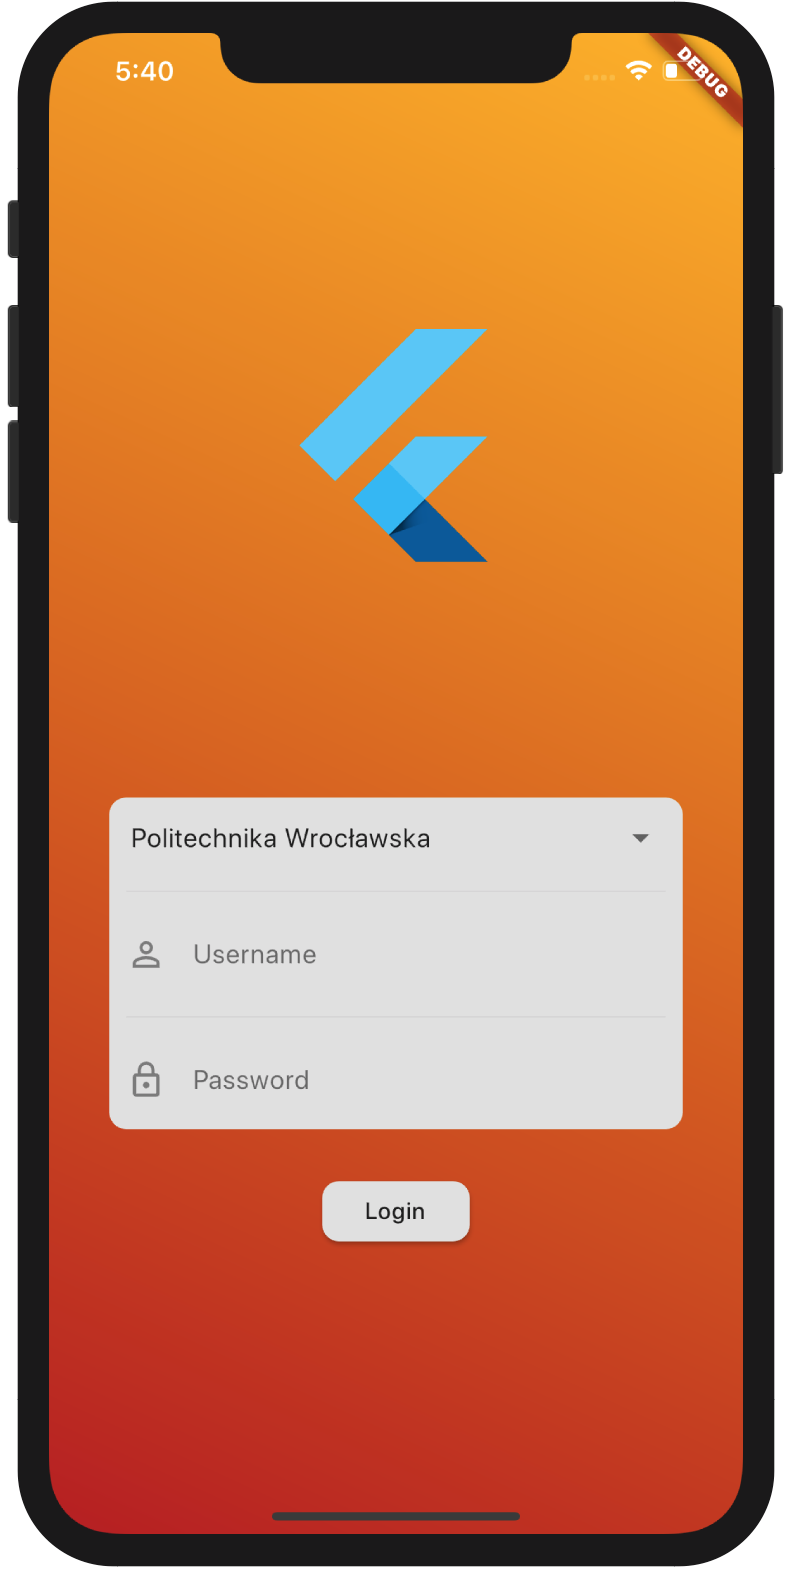
\includegraphics[page=1,width=0.3\textwidth]{fig06/login_page.png}}}} &
        b) & \vtop{\vskip-2ex\hbox{{\includegraphics[page=7,width=0.3\textwidth]{fig06/login_page_dropdown.png}}}} \\
    \end{tabular}
    \caption{Screenshots of the mobile application: a) login page, b) login page with the university drop-down menu} \label{fig:login-dropdown}
\end{figure}

The screen seen by users after they log in is the homepage (Fig.~\ref{fig:home-grades-payments}a). At the top, there are two icons (logout and settings). When users click on the first one, they get logged out of the app. The second one should open a settings tab where users could change some properties. It has not been implemented yet. Also, the default application language is set to English. As of now, the language change functionality has not been implemented.

In the middle, there is a ``Profile'' section where users can see their details like name, student number, university, degree, faculty, subject, and specialization. This segment also contains a~user profile photo retrieved from the system. The next area consists of news from users' faculty and university websites.
All screens, except the login page, have bottom navigation. It allows users to change tabs and quickly see which page they are currently on.

The page shown in Figure~\ref{fig:home-grades-payments}b lists all user grades with their details. On the left side, there is a section with the grade value and number of ECTS credits associated with the class. On the right, starting from the top, there is the class name, date of issue, lecturer, and type of class.

The page presented in Figure~\ref{fig:home-grades-payments}c shows a list of payments related to the current user. Each entry has a value (in Polish złotys), name, date of payment, and status. The number of the installment is an optional property and does not have to occur in every element.

\begin{figure}[t]
    \centering
    \begin{tabular}{@{}l@{}l@{}l@{}l@{}l@{}l@{}}
        a) & \vtop{\vskip-2ex\hbox{{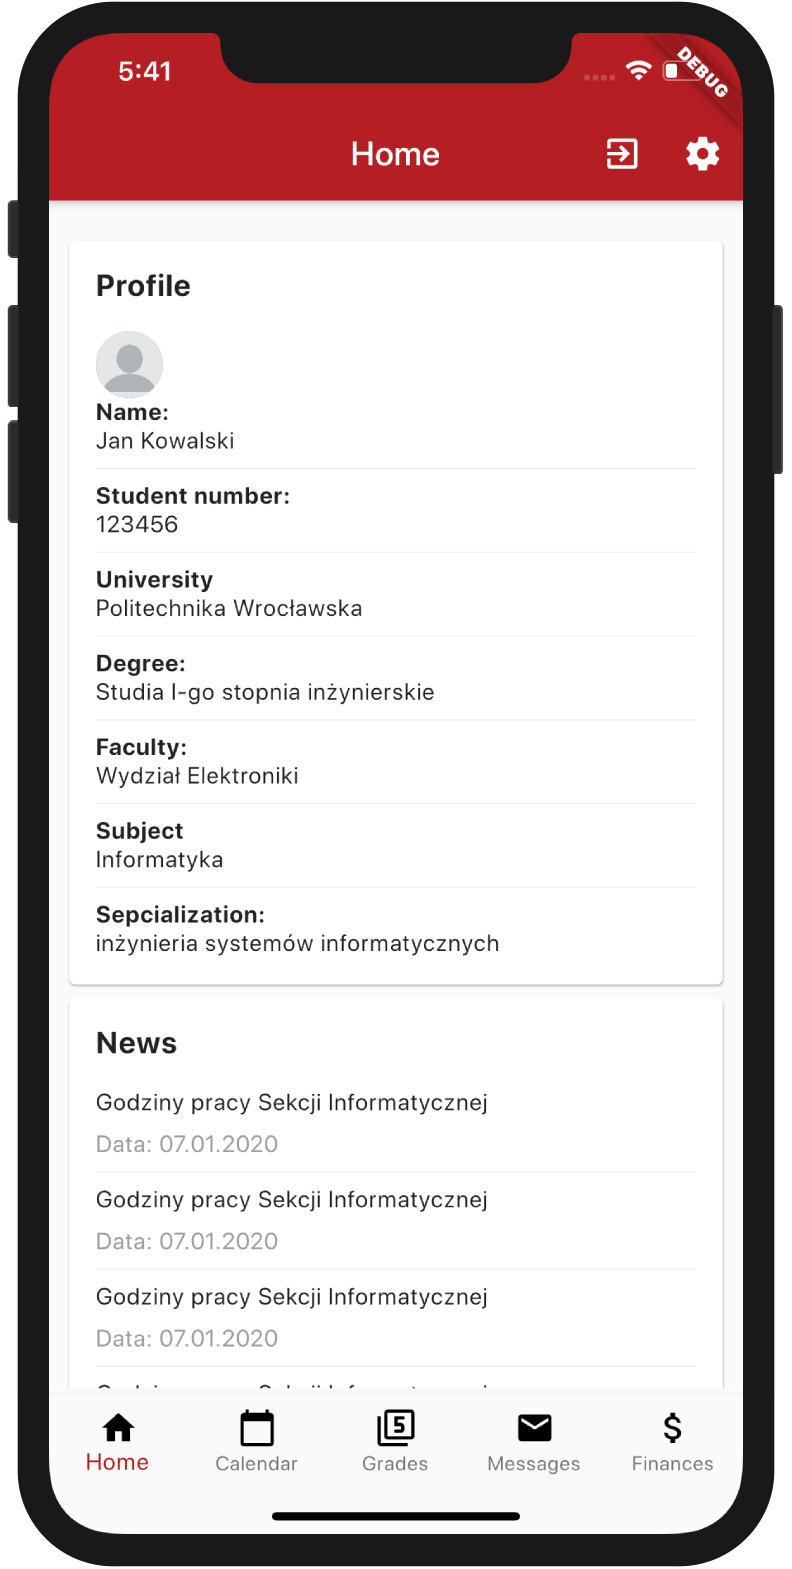
\includegraphics[page=1,width=0.3\textwidth]{fig06/home_page.png}}}} &
        b) & \vtop{\vskip-2ex\hbox{{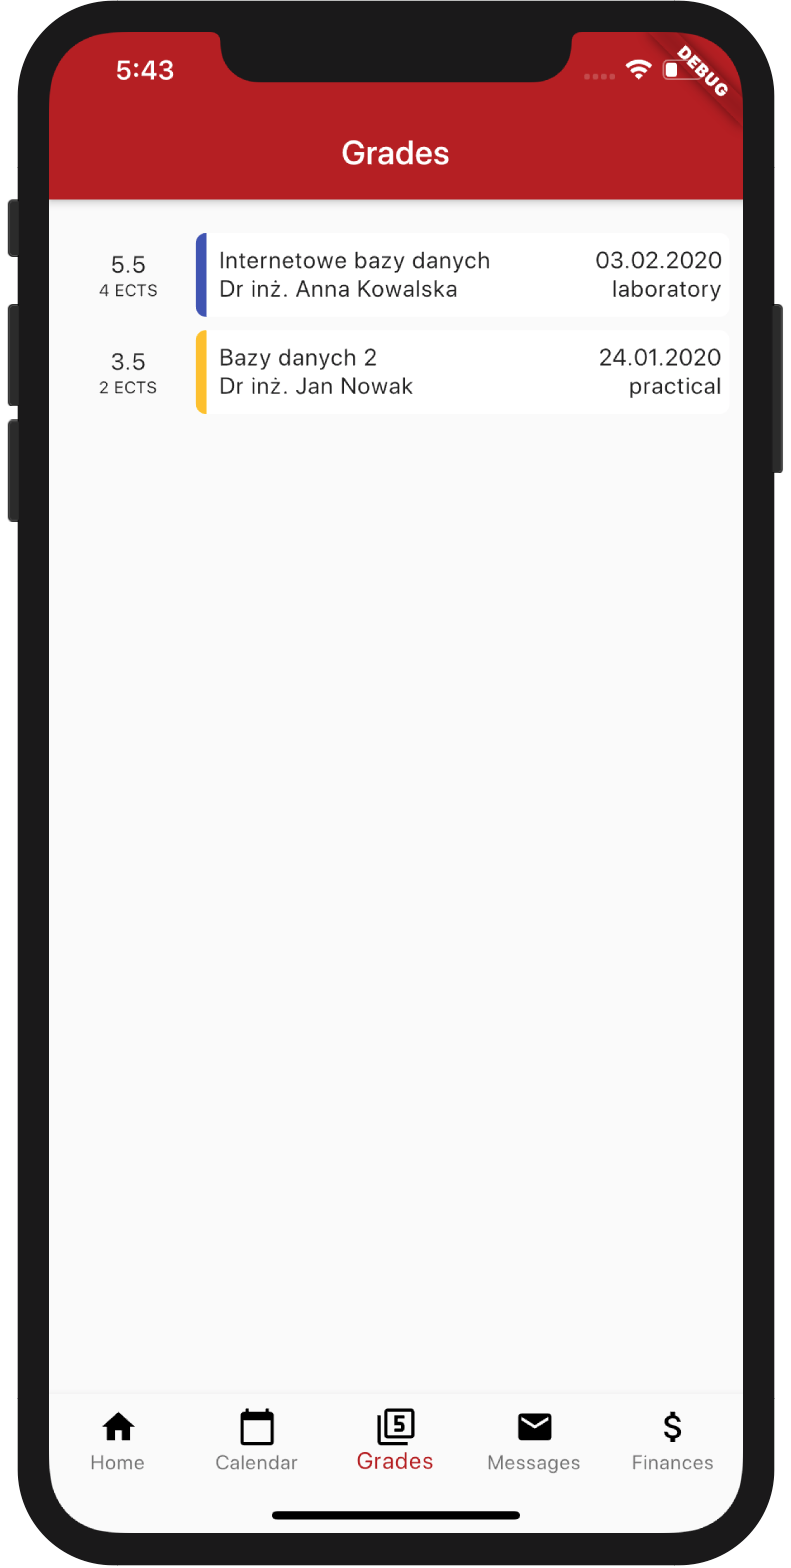
\includegraphics[page=1,width=0.3\textwidth]{fig06/grades_page.png}}}} &
        c) & \vtop{\vskip-2ex\hbox{{\includegraphics[page=7,width=0.3\textwidth]{fig06/payments_page.png}}}} \\
    \end{tabular}
    \caption{Screenshots of the mobile application: a) homepage, b) grades page, c) payments page} \label{fig:home-grades-payments}
\end{figure}

One of the most important screens in the application is the calendar page (Fig.~\ref{fig:calendar-page}). It shows all classes that the user have to attend. The first image (Fig.~\ref{fig:calendar-page}a) does not present any events planned for the selected date. All red numbers indicate that it is a weekend or a holiday. The house at the top right corner means that the university is not working and the user can stay at home instead of going to class.
\begin{figure}[t]
    \centering
    \begin{tabular}{@{}l@{}l@{}l@{}l@{}}
        a) & \vtop{\vskip-2ex\hbox{{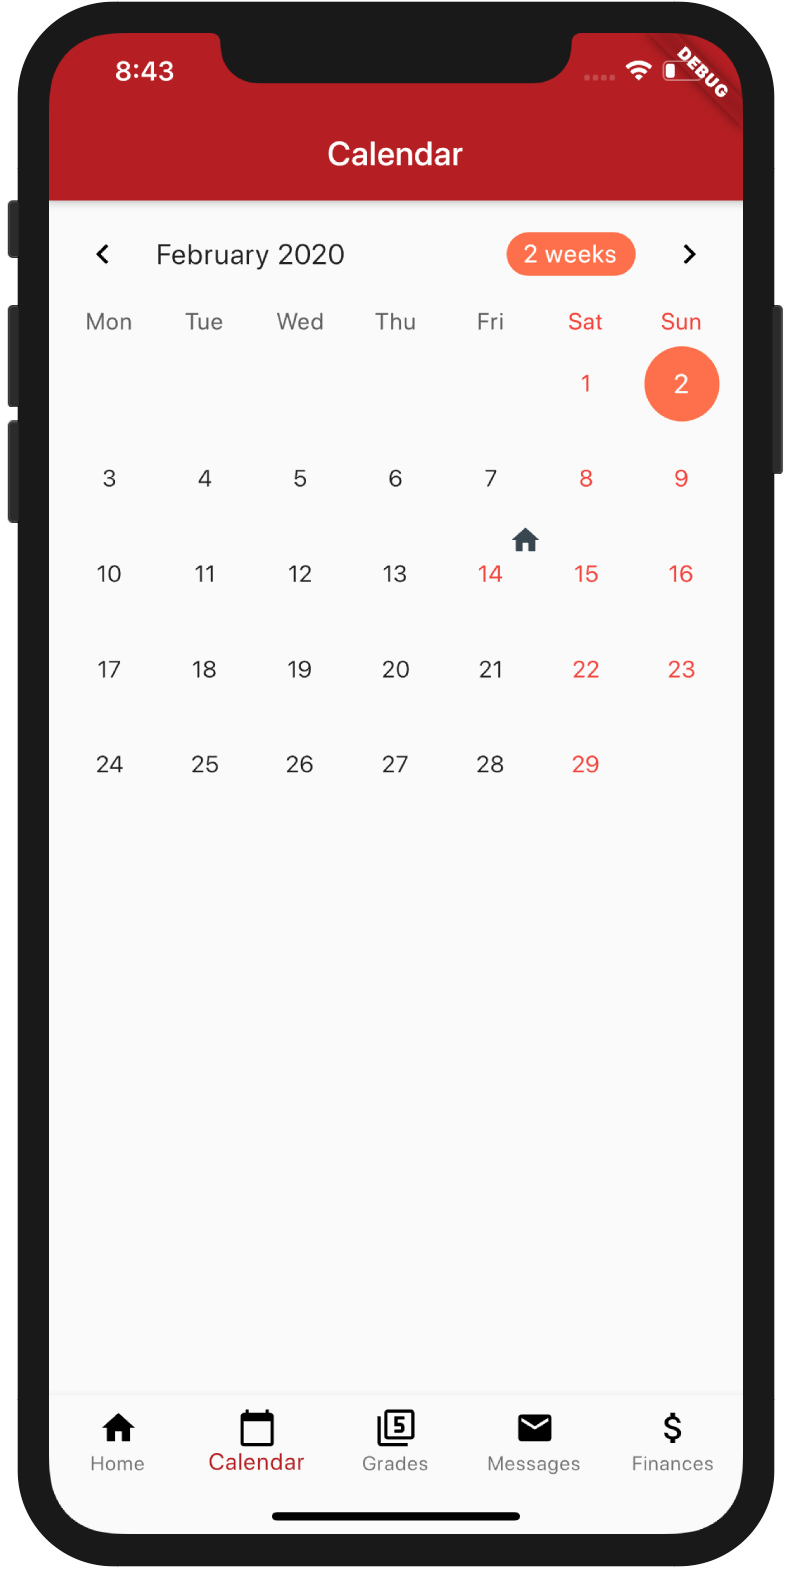
\includegraphics[page=1,width=0.3\textwidth]{fig06/calendar_page_no_classes.png}}}} &
        b) & \vtop{\vskip-2ex\hbox{{\includegraphics[page=7,width=0.3\textwidth]{fig06/calendar_page_with_classes.png}}}} \\
    \end{tabular}
    \caption{Screenshots of the mobile application: a) calendar page with no classes, b) calendar page with available classes} \label{fig:calendar-page}
\end{figure}

The image in Figure~\ref{fig:calendar-page}b shows a different view of the calendar. It can be swapped using the button in the top right corner of the page. There are three available appearances:
\begin{itemize}
    \item one month;
    \item 2 weeks;
    \item a week.
\end{itemize}
 
The indicator in the lower-left corner of a day tells users how many events they have planned. When users select a date, a list of classes appears with details such as the beginning and the end of the class, its name, lecturer, classroom, and type.
The viewed month can be changed by swapping the screen left or right or by clicking on one of the arrows at the top of the page.


The messages page (Fig.~\ref{fig:messages-details-page}a) lists all messages received by users in their university system. On the left-hand side, there is a section displaying specifics like sender, topic, and partial content. On the right, there is a date of receipt. After users select one of the listed messages, they are redirected to a more detailed page (Fig.~\ref{fig:messages-details-page}b) where they can view, in addition to previously seen details, the entire content of the message, and CC recipients.
\begin{figure}[hb]
    \centering
    \begin{tabular}{@{}l@{}l@{}l@{}l@{}}
        a) & \vtop{\vskip-2ex\hbox{{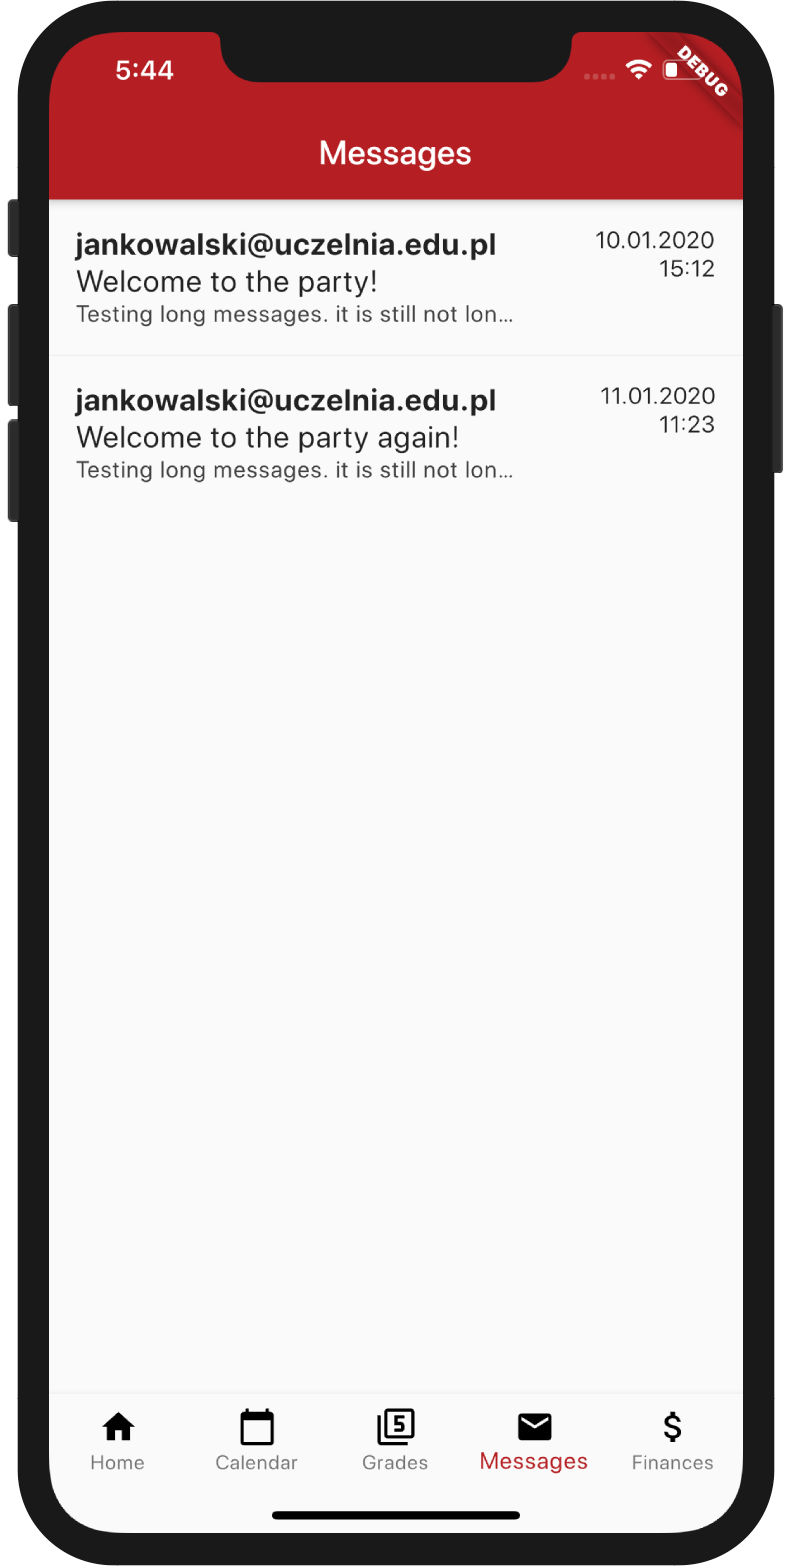
\includegraphics[page=1,width=0.3\textwidth]{fig06/messages_page.png}}}} &
        b) & \vtop{\vskip-2ex\hbox{{\includegraphics[page=7,width=0.3\textwidth]{fig06/message_details_page.png}}}} \\
    \end{tabular}
    \caption{Screenshots of the mobile application: a) messages page, b) message details page} \label{fig:messages-details-page}
\end{figure}
